48. \begin{figure}[ht!]
\center{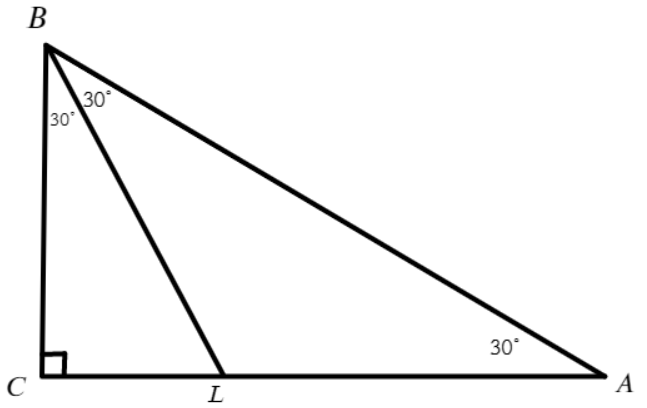
\includegraphics[scale=0.35]{g48.png}}
\end{figure}\\
Если внешний угол при вершине $B$ равен $120^\circ,$ то $\angle B=180^\circ-120^\circ=60^\circ.$ Тогда $\angle A=90^\circ-60^\circ=30^\circ$ и $\angle CBL=\angle LBA=30^\circ$ (так как $BL$ --- биссектриса). В прямоугольном треугольнике $CBL$ катет $CL$ лежит напротив угла в $30^\circ,$ поэтому $CL=\frac{1}{2}BL=\frac{1}{2}\cdot2=1$см. В треугольнике $LBA$ углы при стороне $BA$ равны, значит он равнобедренный и $AL=BL=2$см. Таким образом, $AC=CL+AL=1+2=3$см.\\
